\chapter{Introduction}
\addcontentsline{toc}{chapter}{\textbf{Introduction}}

Humanity is amidst a critical ecological era, whereby the ecological thresholds of the earth system have been crossed. The notion of \textit{planetary boundaries} \citep{rockstrom2009safe,steffen_2015_planetary} illustrates how the anthroposphere, the planetary-scale effects of human activities, have become an additional functional component and are capable of changing the Earth system \citep{richardson_earth_2023} alongside the geopshere (energy flow and nonliving materials in Earth and atmosphere) and biosphere (all living organisms/ecosystems). The "planetary boundaries" framework identifies the limits to the impact of the anthroposphere on the Earth system that can safeguard Earth's interglacial state - the only one where civilization is known - by identifying a "safe operating space". Among these nine boundaries, \cite{richardson_earth_2023} estimate that 6 have been crossed, threatening the stability and resilience of the Earth system. 

\begin{figure}[h]
	\centering
	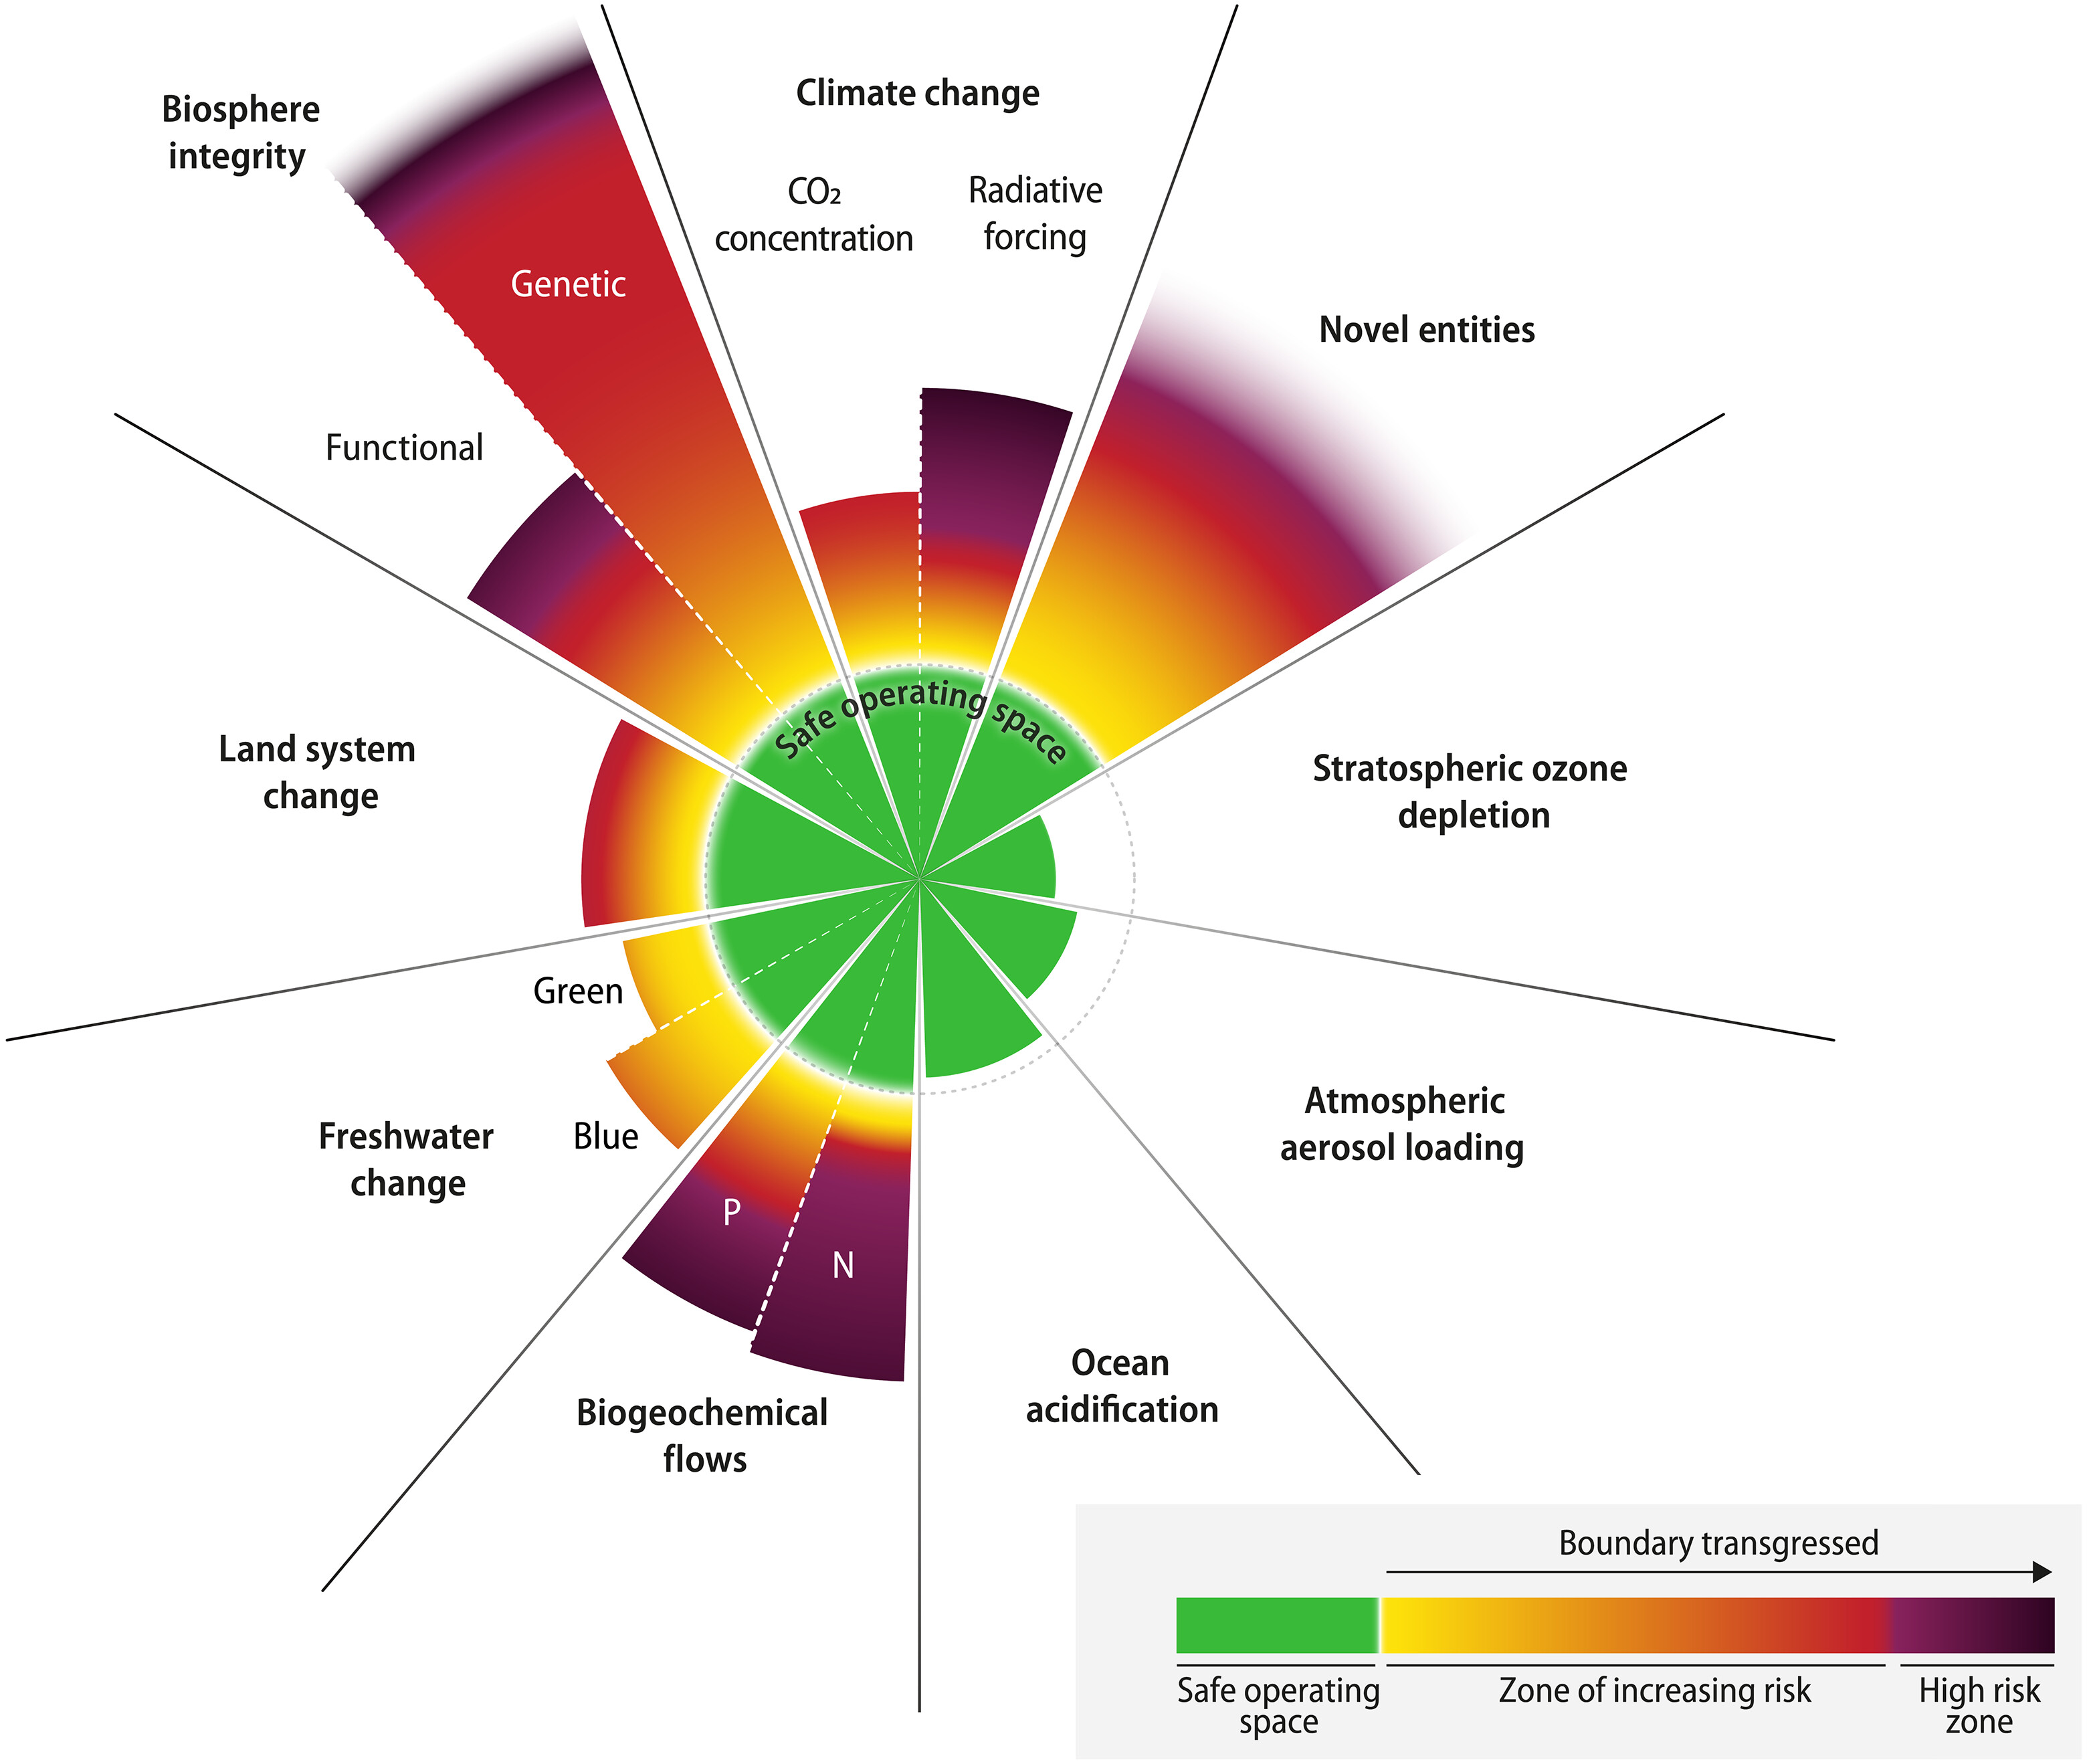
\includegraphics[width= .7\textwidth]{figures/intro/planetary_bounds.jpg}
	\caption{Current status of control variables for all nine planetary boundaries, from \cite{richardson_earth_2023}}
\end{figure}

Among these planetary limits, the integrity of the biosphere has gradually become of particular interest, along with its interaction with other limits, such as climate change, or novel entities (including pollution). Created in 2012, the Interdisciplinary Panel on Biodiversity and Ecosystem Services (IPBES) has been raising the alarm on the state of "Nature" globally. Its chair, Sir Robert Watson, put it clearly\footnote{See the \href{https://www.ipbes.net/news/Media-Release-Global-Assessment}{press release address of the 2019 report}}:
\begin{displayquote}
"\textit{The overwhelming evidence of the \cite{ipbes_2022_6417333} Global Assessment from a wide range of different fields of knowledge, presents an ominous picture [...]. The health of ecosystems on which we and other species depend is deterioriating more rapidly than ever. We are eroding the foundations of our economies, livelihoods, food security, health and quality of life worldwide}"
\end{displayquote}

"Nature" is a central concept in the IPBES framework \citep{ipbes_2022_6417333}:

\begin{displayquote}
\textit{Nature (also defined as living nature) [is] the nonhuman world, including coproduced features, with particular emphasis on living organisms, their diversity, their interactions among themselves, and with their abiotic environment. Within the framing of natural sciences, nature includes e.g. all dimensions of biodiversity, species, genotypes, populations, ecosystems, the biosphere, ecosystem functioning, communities, biomes, Earth life support's systems and their asosicated ecological, evolutionary, biogeochemical processes and biocultural diversity. Within the framework of economics, it includes categories such as biotic natural resources, natural capital, and natural assets. Within a wider context of social sciences and humanities and interdisciplinary environmental sciences, it is referred to with categories such as natural heritage, living environment, or the nonhuman. Within the context of other knowledge systems, it includes categories such as Mother Earth [...], Pachammama [...]}\\
\hspace*{\fill} \small{\cite{ipbes_2022_6417333}, p.14, see also \cite{DIAZ20151}}
\end{displayquote}

Nature, as defined in this approach, is a very large and complex object.
It is defined across ontological and epistemological differences (living and non-living e.g. matter), different types of interactions, at various scales (genotypes v. ecosystems), at different types of processes (biological v. ecological), and across different fields of inquiry (natural sciences v. social sciences). In this dissertation, I study more specifically "biodiversity", which focuses on the variability among living organisms. While it is itself an ambiguous concept, biodiversity tends to put the focus on living organisms, in relation to their material, biotic and abiotic environment (as opposed to the study of the non-living environment) and on its critical role among other components of the Earth system.

The \cite{ipbes_2022_6417333} report documents the drastic changes the biosphere is going through and considers these changes through an \textit{anthropocentric} lense, e.g. mediating the aforementioned changes through the multiple and diverse contributions that Nature and biodiversity bring to people. It stresses how disruption impacts human lives and highlights the role of anthropogenic (e.g. of human origin) drivers of the disruption of Nature and biodiversity. 
 
This reports sets different objectives to scientific research. The first objective is to explain the feedback mechanisms : how do human livelihoods impact biodiversity? In response, how does biodiversity impact human livelihoods? This objective involves understanding the causes and measuring the direct and indirect anthropogenic drivers of change in Nature and biodiversity on the one hand, and on the other hand understanding the channels and scales through which Nature and biodiversity contribute to human livelihoods, as well as measuring these contributions. Hence, studying the demise of nature, and the potential to remedy it calls for an integrated perspective, that joins natural sciences to social sciences, through frameworks such as social-ecological systems \citep{Ostrom2009}. 
\\
The second objective is to provide a framework to assess the desirability, the feasibility and means of implementation of collective pathways that would remedy the crisis nature is facing. In a way, it involves designing and implementing policy pathways towards sustainable futures, e.g. finding definite courses or methods of action selected from alternatives, at the individual, collective or governmental levels, to achieve future states of the world which remain in a safe operating space regarding planetary bounds \citep{rockstrom2009safe,steffen_2015_planetary}.

In this dissertation, I take on these two objectives using a framework stemming from economics and ecology. A first version of the research questions this thesis aims at solving is: 
\begin{enumerate}
\setlength{\itemsep}{0pt} % No space between items
\item What are the feedback relationships between biodiversity and antropogenic drivers of its decline? 
\item What underlying mechanisms must policy pathways tackle to remedy this demise?
\item  How can integrated economic and ecological approaches be used and refined to analyze inform and design policies? 
\end{enumerate}

In order to refine these questions, I first define the concept of biodiversity, through its natural and social sciences appraisals, and highlight ongoing trends in its demise.


\subsection*{Emergence and definition of biodiversity as an ecological concept}
\addcontentsline{toc}{section}{Emergence and definition of biodiversity as an ecological concept}

Biodiversity emerged as a concept in the 1980s, along with the emergence of "conservation biology", a branch of biology concerned with the protection of "biological diversity" \citep{soule_what_1985}, as a response to an acceleration in the loss of species. The moral stance of conservation biologoy is that species should be protected for their own sake \citep{soule_conservation_1986}, they have intrinsic value. 
The concept of biodiversity is therefore embedded in an ethical judgement and a call for action. In the wake of the 1992 Rio United Conference on Environment and Development, the \href{Convention on Biological Diversity}{https://www.cbd.int/} emerged as an international treaty to safeguard biodiversity. In doing so, it provided an internationally agreed upon definition:

\begin{displayquote}
"\textit{"Biological diversity" means the variability among living organisms from all sources including, inter alia, terrestrial, marine and other aquatic ecosystems and the ecological complexes of which they are part; this includes diversity within species, between species and of ecosystems.}"\\
\hspace*{\fill} \small{\href{https://www.cbd.int/convention/articles/default.shtml?a=cbd-02}{Article 2 of the Convention on Biological Diversity}}
\end{displayquote}

This definition highlights a key differentiating feature from other parts of nature, e.g. the living nature of the objects of study. Compared to abiotic factors, biological diversity is characterized by intrinsic growth, reproduction and metabolism (at the individual and population levels), and evolution (at the genetic, and species level). Additionally, these rates of change through time are commensurable with human experience, and most processes (e.g. reproduction, population collapse or recovery, genetic evolution) can be observed within a human lifetime as opposed to the geological temporal scale. 

As highlighted by \cite{VanDyke2008} and \cite{mouysset_diversity_2023}, the definition of biodiversity is difficult, as it recovers ethical, conceptual and measurement dimensions. Biodiversity can be viewed as "an intrinsic, value-ladden quality of natural systems that should be preserved for its own sake" \citep{VanDyke2008, mouysset_diversity_2023}, but it also refers to measurable features.
% relevant to understanding genetic distribution, population levels, community structure (e.g assembly of interacting species in a given area), environmental processes, and ecosystem functions (e.g. the ecological processes performed by living organisms, such as carbon sequestration, nutrient recycling, water filtration etc). 
This definition implies different scales from a hierarchical perspective, at the genetic level, at the species, the community, and the ecosystem levels (defined as the interaction of communities and their abiotic environment). These levels imply different forms of measurement, including the distribution of genes, species abundance (e.g. the number of individuals in a population, at a given time and location), species richness (e.g. the number of different species, at a given time and location) within communities, among communities, and across larger scales (e.g. alpha, beta and gamma diversities.), as well as variations in the abiotic factors that form ecosystems, such as temperature, humidity, water quality, soil quality etc. 
It also comprises different types of diversity : structural diversity (for example, the layers of canopy in forests, the sex-ratio in animal populations), compositional diversity (the variety and abundance of species within a community), and functional diversity (variety of environmental processes performed by living organisms in a given area e.g. carbon sequestration, nutrient cycling or seed dispersal, see \cite{loreau_biodiversity_2002})

\begin{figure}
	\centering
	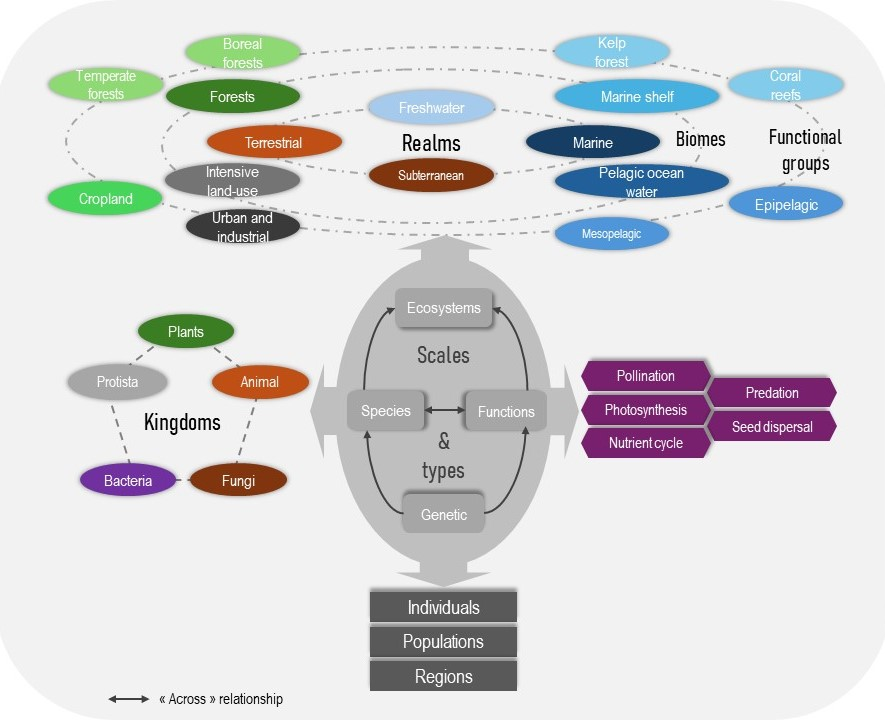
\includegraphics[width =.8\textwidth]{figures/intro/biodiv_illustration.jpg}
	\caption{Biodiversity : a multiform concept across scales and types}
	\label{fig:intro_biod}
\end{figure}

\cite{mouysset_diversity_2023} highlights the difficulty of articulating the definition with common levels in scientific analysis e.g. genetic, taxonomic, and ecosystem, as biodiversity level can fall in between: "populations may be considered from a genetic and taxonomic perspective, or communities that fall between the taxonomic and ecosystem levels". Additionally, as structural and compositional diversity can be seen as the source of functional diversity, the different classes of diversity may be difficult to work with given their colinearity. 

The multiple dimensions of biodiversity highlight several of its critical features. First, it is impossible to measure biodiversity with a single indicator. The study of biodiversity requires multiple indicators to integrally assess the evolution of biodiversity, across scales and types of diversity. The emergence of the concept responds to a desire to protect biodiversity for its own, but also humanity's sake. 

\clearpage
\subsection*{Nature's Contributions to People: rationales for biodiversity conservation}
\addcontentsline{toc}{section}{Nature's Contributions to People: rationales for biodiversity conservation}


Originally descriptive, ecosystem functions were increasingly viewed from a human perspective starting in the 1970s \citep{hueting1969functions, schumacher1973small}, evolving into the concept of ecosystem services \citep{ehrlich1981extinction} to illustrate biodiversity loss consequences \citep{gomez_history_2010}. This marked a shift from intrinsic to anthropocentric (e.g. given by humans) value \citep{mouysset_diversity_2023}, recognizing biodiversity’s instrumental and relational values—serving human ends and fostering meaningful relationships. Gradually, biodiversity had to be protected for its role in sustaining human life.


%While originally descriptive, ecosystem functions have gradually been referred to from the human point of view (starting in the 1970s, see  \cite{hueting1969functions, schumacher1973small}) and how these functions served human societies, through the concept of \textit{ecosystem services} \citep{ehrlich1981extinction}, as a pedagogical tool to illustrate the consequences of biodiversity loss \citep{gomez_history_2010}.  In this respect, a value switch was operated from an intrinsic value towards an anthropocentric value (e.g. given by humans) standpoint \citep{mouysset_diversity_2023}. In more details, biodiversity features an instrumental value (e.g. serves to achieve a human end) and a relational value (e.g. the importance of desirable, meaningful, and often reciprocal relationships - beyond means to an end) : if biodiversity is to be preserved, it is because of the functions it performs that sustain and improve human life.

The concept gradually gained traction in academic research, and as \cite{Costanza1997} quantified the value of natural capital and ecosystem services, at a staggering 33 trilion \$USD, amounting to approximately 30\% of the 2020 World GDP, the concept reached the policy arena. In 2005, the Millenium Ecosystem Assessment \citep{MEA2005} placed ecosystem services at the center of the policy agenda : it emphasized an anthropocentric value of ecosystem services, but established a dependence of human societies on ecosystem services, and further, on the functioning of ecosystem. In this respect, the Millenium Ecosystem Assessment \cite{MEA2005} was a landmark in safeguarding biodiversity through a \textit{strong sustainability} paradigm (see box 1), and triggered the operationalization of the concept into policy at a large scale (which I will develop later on). The ecosystem services framework was divided into 4 categories, relating to the specific type of services contributing to "human wellbeing" : supporting services (e.g. services allowing for other ecosystem services to be present, including nutrient cycling and primary production) and regulating services ("benefits obtained from the regulation of ecosystem processes" e.g pollination, waste decomposition etc); cultural services ("the nonmaterial benefits people obtain from ecosystems through spiritual enrichment, cognitive development") and provisioning services ("all the products obtained from ecosystems",\cite{MEA2005}, p.54)

\begin{figure}[h]
	\centering
	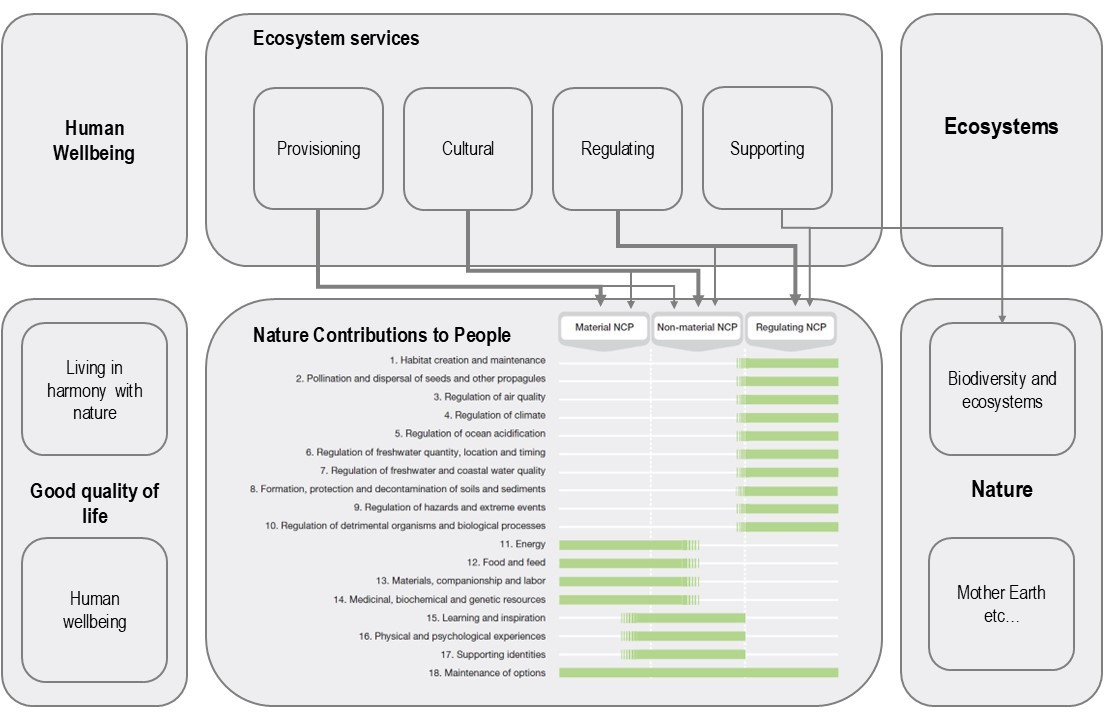
\includegraphics[width = \textwidth]{figures/intro/NCPs2.jpg}
	\caption{Description of the 18 Nature Contribution to People and the connection between the NCP framework \citep{ipbes_2022_6417333} and the Ecosystem Services Framework \citep{millennium2005ecosystems}}
	\subcaption*{Adapted from \cite{diaz_2018} and \cite{ipbes_2022_6417333}}
\end{figure}

Recently, the IPBES platform moved onto a new conceptual framework highlighting Nature Contributions to People (NCP) \citep{DIAZ20151}, defined as "all the contributions, positive and negative, of living nature [...] to people's quality of life \citep{diaz_2018}". This framework underpins 3 types of contributions to people: material contributions to people (flows from nature to people typically consumed to "operate a society or enterprise" (IPBES, p.16), non material contributions (eg. nature's effects on "subjective and psychological aspects underpinning peoples quality of life) and regulating contributions (e.g. "functional and strcutrual aspects of organisms and ecosystems that modify the environmental conditions experienced by people and/or regulate the generation of material and non material contributions"). This framework highlights how Nature Contributions to People can be positive or negative, and depend on the spatial and temporal definition of the contribution, as a given entity can be at the same time the source of positive and negative contributions: for example, forests foster habitat, but also risk endangering people in the event of wildfires. Additionally, it provides a more encompassing view than ecosystem services, as it encompasses perspectives ranging from biodiversity as natural capital employed in an ecological production function (see \cite{polasky_integrating_2009} for a review), as well as perspectives where biodiversity has agency and is linked by reciprocal care obligations to humans \citep{descola}. 

A multifaceted correspondence between the different components and dimensions of biodiversity and its contributions to people underpin human livelihood. The global decline of biodiversity threatens NCPs.

\clearpage
\begin{tcolorbox}[breakable, 
colback=verylightgray, 
colframe=gray!75!black, 
title= {Box 1 - Weak v. Strong Sustainability},
%code={\singlespacing},
fontupper=\small]
\par % This \par ensures spacing before the text starts
\justifying % Start justified text

In 1987, the release of the Brundtland Report \citep{brundtland} provided a broad definition of sustainable development: 

\begin{displayquote}
\textit{"In essence, sustainable development is a process of change in which the exploitation of
resources, the direction of investments, the orientation of technological development; and institutional change are all in harmony and enhance both current and future potential to meet human needs and aspirations"}\\
\small{\cite{brundtland}, p.43}
\end{displayquote}

Implementing sustainable development remained an open question. In economics, a "weak sustainability perspective", pioneered by works of \cite{hartwick_intergenerational_1977} and \cite{solow_intergenerational_1986} on exhaustible resources, suggested that "maintaining a non-declining capital stock,which allegedly could be put into practice by investing in manufactured capital all the rents derived from the exploitation of non-renewable natural resources" \citep{gomez_history_2010}. In this approach, natural capital could be integrally substituted by human made capital. On the other hand, the "strong sustainability" approach advocates advocates for a complementarity, rather than substitutability of resources \citep{costanza_daly}, acknowledging the dependence of humans on ecosystems
\end{tcolorbox}


\subsection*{Decline in biodiversity : trends and drivers}
\addcontentsline{toc}{section}{Decline in biodiversity : trends and drivers}

Biodiversity metrics are declinning across all the scales of analysis. The structural conditions of ecosystems, the compositions of ecological communities and populations of species have experienced dramatic changes.\\
The share of unchanged, protected wildlife habitat has plumetted on both land and sea \citep{watson_2016_catastrophic, jones_2018_location} to 23\% and 12\% of space, respectively. At the community level, the share of originally present biodiversity falls bellow 90\% across all biomes, \citep{Hill311787} and local communities are becoming more and more similar \citep{mckinney_1999_biotic}, driven by the increased extent of animal and plant non-alien invasive species, rising by 13\% per decade \citep{seebens_no_2017}. At the species level, to date, global species richness is threatened by a mass extinction, as the global rate of species extinction is at least ten times higher than the average rate over the past 10 million years and is accelerating \citep{barnosky_has_2011, ceballos_accelerated_2015}. On average, 25\% of species are currently threatened with global extinction across a wide range of plant and animal species, on land and at sea \citep{IUCN_redlist_2024}. Using habitat based methods\footnote{ The IUCN Redlist uses detailed accounts for species, in a bottom-up approach, to analyze the extinction risk of species. A top-down approach, relying on the evolution of available habitat and the species-area relationship, uses changes in land use to forecast the extinction of species in a more aggregate manner \citep{Diamond1972BiogeographicKE}}, \cite{Hoskins309377} find that hundreds of thousands of plant and animal species are threatened, and will repay the \textit{extinction debt} caused by anthropogenic changes to their habitats : only 92.1\% of terrestrial vertebrate species, 91.6\% of terrestiral invertebrates and 90.7\% of terrestrial plants have enough habitat to persist. These results suggest that around half a million terrestrial animal and plant species - including over 3000 vertebrates and over 40,000 plants - \textit{dead species walking}, doomed to become extinct, unless their habitats improve in time to prevent it \citep{ipbes_2022_6417333}.

%\begin{figure}[h]
%    \centering
%    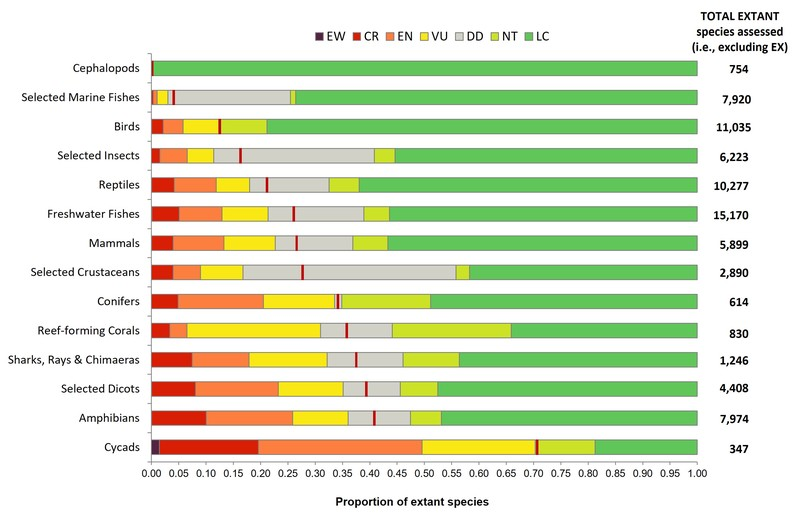
\includegraphics[width=0.8\linewidth]{figures/intro/IUCN_redlist}
%    \caption{The proportion of extant (i.e., excluding Extinct) species in \citet{IUCN_redlist_2024}}
%    \subcaption*{Assessed in each category for the more comprehensively assessed (i.e., at least 80\% of the group has been assessed) groups containing $\geq$ 150 species. Species are grouped into classes. The numbers to the right of each bar represent the total number of extant species assessed for each group. \textbf{EW} - Extinct in the Wild, \textbf{CR} - Critically Endangered,\textbf{ EN} - Endangered, \textbf{VU} - Vulnerable, \textbf{NT} - Near Threatened, \textbf{DD} - Data Deficient, \textbf{LC} - Least Concern.}
%    \label{fig:intro_iucn}
%\end{figure}

Drivers of biodiversity decline are of anthropogenic origin. They can be classified between \textit{direct} drivers, e.g. that directly flow form human actions, such as land use change, anthropogenic climate change, overexploitation, and \textit{indirect} drivers, that can be viewed as the root cause for direct drivers, such as  , changes in the value systems that underpin nature uses (\cite{ipbes_2022_6417333} p.55), demography (urbanization and migration), technology, economy (sectoral transitions, trade expansion) and governance (including risht systems for access to resources).

%The Essential Biodiversity Variables framework \citep{pereira_essential_2013} aggregates fine gridded spatial data into 
A synthesis of natural sciences performed by \cite{ipbes_2022_6417333} outlines the roles of principal drivers at the global scale and across realms (see figure \ref{fig:intro_impacts}).
It shows that land and sea use, reefering to the loss, fragmentation\footnote{Undoubtedly, habitat loss is the main driver of terrestrial biodiversity decline. The effects of fragmentation on biodiversity are highly debated. From a theoretical perspective, models have been developed to study the evolution of populations and communities through space and time, e.g. metapopulation and metacommunity models. Theoretical insights highlight that habitat fragmentation increase the extinction risk, and lower colonization probability, resulting in lower survival and diversity \citep{adler_persistence_1994,hill_habitat_1999, thompson_loss_2017}. At the community scale, increases in diversity among communities (e.g. beta diversity) can emerge from different species resource requirements and the larger spatial extent, hence encompassing more environmental heterogeneity, that results from fragmentation \citep{lasky_reserve_2013, chisholm_species_2018}. However, these effects dampen as habitat loss decreases.  
However, at the empirical level, the effect of fragmentation is highly debated. According to \cite{fahrig_ecological_2017}, there is no empirical evidence that a group of small habitat patches generally has lower evological value than large patches of the same total area. Evidence is however found to show that fragmentation does not reduce habitat connectivity, as functional connectivity is improved (e.g. species are in contact with more different resource patches, thus improving the overall functionning). The debate between \citep{fletcher_is_2018} and \citep{fahrig_habitat_2019} surrounds critics based on the ability of statistical models to encompass the effect of fragmentation when habitat loss is present \citep{ruffell_accounting_2016}. Moreover, it reflects the difficulty of landscape ecology, as different mechanisms across scales e.g. patch, landscape and study region, and measures, such as patch size, patch isolation (e.g. distance across patches) and distance to patch edge (e.g. distance to edge within the patch) interact with possible non-linear interactions.}
%
and degradation of wildlife habitat are responsible for 30\% of the impacts on biodiversity. The direct exploitation of wildlife, wild plants and trees represents 23\% of impacts. Climate change, through shifts in biogeographic conditions and changes in habit, impacts on species traits and genetic evolution represents 14\%, and pollution represents 14\% of impacts. Finally invasive alien species represent 11\%. These drivers have differenciated impacts across ecosystems and biomes \citep{ipbes_2022_6417333}. 

\begin{figure}[h]
	\centering
	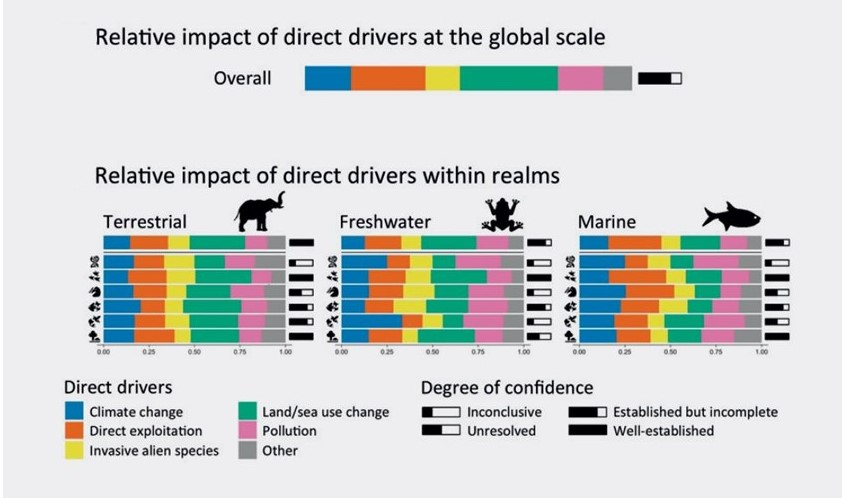
\includegraphics[width = .95 \textwidth]{figures/intro/intro_impactsfin.jpg}
	\caption{Aggregate and realms specific impacts of anthropogenic direct drivers of biodiversity decline adapted from \citep{ipbes_2022_6417333}}
	\label{fig:intro_impacts}
\end{figure}

On land, land use change is the most important driver (30.5\%), driven by deforestation and agriculture, and direct exploitation follows next (21\%). Tropical and subtropical dry and humid forest host the greatest biological diversity. For example, they host the 10 hotspots with the greatest total number of vertebrates \citep{mittermeier_global_2011}. In such forests, habitat loss and degradation are the main drivers of reductions in species abundance and richness \citep{newbold_global_2014}. Legal and illegal selective logging destroy habitat \citep{hoare2022establishing,  bousfield_2023_large} and are combined with hunting and poaching of wildlife \citep{gallego_2020_combined}, generating between 60 and 180 billions  \$ USD of revenue \citep{gfi_2017}\footnote{Illegal wildlife trade represents between 5 and 23 billion \$USD, while illegal logging represents 52 to 157 billion \$USD}. 

For marine species, overexploitation is the main driver (29\%) \citep{ipbes_2022_6417333}. With 90 million tons of capture  (and 141 billion \$ USD)  in 2020 \citep{fao_2022_state}, fisheries stock within biologically sustainable levels have decreased to 64.6\% in 2019, from 90\% in 1974\footnote{ In this calculation, all fishery stocks are equally counted, irrespective of their abundance or catch}, driven by overfishing in the Southeast Pacific and the Mediterranean and Black seas. Nonetheless, illegal, unreported and unregulated (IUU) fishing is a threat to fisheries. Estimates from 15 years ago \citep{agnew_estimating_2009} estimated it represented between 11 and 26 million tonnes of fis with a value of 10 to 23 billion \$ USD. 
 
Additionally, anthropogenic climate change drives ecosystem disruptions on land \citep{burrell_anthropogenic_2020, conradi_reassessment_2024} and at sea \citep{gomes_marine_2024}, through changes in various channels including ecological suitability and foodweb disturbances. On land, for example, mediterranean forests, wooldlands and scrubs, covering 4 million km$^2$, are areas of exceptionally high diversity too \citep{Mooney2001, blondel_2010}, threatened with urban expansion and increased wildfire risk. Wildfire frequency and severity are expected to increase with global warming \citep{Dupuy2019ClimateCI}, causing important direct and indirect costs to society including destruction of infrastructure and perturbations to economic activity \citep{wang_economic_2021}, smoke related health conditions \citep{burke_wildfire_2023, heft-neal_behavior_2023}, disrupting structural features of ecosystems \citep{Ayars2023} and threatening biological diversity \citep{Wintle2020}.



\subsection*{Economic challenges to remedying the drivers of decline}
\addcontentsline{toc}{section}{Economic challenges to remedying the drivers of decline}

Habitat loss and overexploitation present both common and differentiated challenges. A common identifiable cause is the large opportunity cost of preserving a species habitat, or existence, in the presence of other economic alternatives for land and time, as well as financial constraints. Additionally, habitat loss and overexploitation share a temporal dynamic aspect, where immediate actions have durable consequences, possibly irreversible.

Habitat loss and fragmentation in terrestrial ecosystems present specific challenges. Forests, for example, serve multiple uses (or NCPs) by various agents: loggers profit from timber, settlers clear land for agriculture, hikers seek pristine landscapes, and conservationists aim to restore natural cycles. Forests also hold spiritual and cultural value, creating conflicts among these uses. For instance, deforestation destroys both habitat and sacred land, while wildfire prevention can damage wildlife habitat. Species can also have mixed impacts; deer, for example, are valued at low densities but cause damage at higher densities \citep{putman_identifying_2011}. 
%Climate change worsens habitat loss by altering habitat distribution and increasing threats like wildfires \citep{Dupuy2019ClimateCI,wasserman_climate_2023}\\
A second key feature to halt habitat fragmentation is considering the integral set of interdependencies, ecological spillovers and economic externalities that underlie the spatial dimension. The configuration of space, and species movement is at least partly the result of an economic decision. Maintaining habitat connectivity involves identifying patches and paths to be conserved or restored that contribute most to it, in the form of corridors, ecoducts or stepping stones \citep{Turner2005, Turner2011}. The value of patches and paths for connectivity is intrinsically linked to their surrounding : at the same geographic location, a patch has differential value for biodiversity habitat if it is connected to others, or if it is isolated (see box 3). When paths are beyond human control, patches have different importance based on their location, and when the location of patches is fixed, the extent of paths and their location is paramount.
\\
Third, as multiple actions and uses structure connected elements of ecosystems (e.g. different tracts of land, or different biodiversity scales), they trigger spatial spillovers e.g. consequences that go beyond their \textit{in situ} effects. When these spillovers are not taken into account by the agents that generate them, they can be called "dynamic spatial externalities" \citep{sanchirico_bioeconomics_1999, costello_optimal_2008, costello_private_2017}. As halting habitat loss and fragmentation involves conserving tracts of land, neighboring parties may very well benefit (or suffer) from more wildlife and ecosystem (dis-)services on their property, through time. These externalities can trigger specific problems of "race to the bottom" \citep{costello_private_2017} : when neighboring parties of a decision maker that undertakes conservation, or risk reduction, fail fail to reciprocate as they benefit from spillovers, a vicious circle of least action is triggered. Conversely, when ecological spillovers are positive, this may lead everybody to use a resource at unsustainable levels, even in the presence of well defined rights, absent other mechanisms \citep{janmaat_sharing_2005,kaffine_unitization_2010}. Hence, habitat fragmentation and overexploitation are interrelated through spatial connectivity. 
\\
Fourth, improving habitat loss and fragmentation involves coordinating numerous actors towards increasing the area and connectivity of habitat, while taking into account the associated costs and benefits. In some cases, the financial constraints, the magnitude of costs associated with increased habitat connectivity and the difficulty of coordination warrant a public policy where a central planner undertakes the action \citep{Mouysset2012}. On the other hand, mechanisms to decentralize efficient spatial planning exist and can be efficient under limited costs of cooperation \citep{bareille_agglomeration_2023}.
 
	Halting overexploitation requires understanding and addressing its motives. Overexploitation (or under control, for pests), results from an imbalance between the appropriation and incumbance of Nature's contributions to people (both positive and negative) and the socially desirable level and allocation of these contributions. 	
	The common nature of most natural resources \citep{Gordon1954, smith_models_1969} has long been identified as one of key reason for their demise: numerous events have shown a "race to the bottom", where the absence of secure property rights hastened the overharvest and decline of populations. It has long been the center of attention, and mechanisms relying on property rights assignment have been studied extensively \citep{libecap_tragedy_2009,costello_partial_2015 isaksen_tragedy_2019}.\\
	

\begin{tcolorbox}[breakable, 
colback =verylightgray, 
colframe=gray!75!black,
title={Box 2 - Habitat Loss, Fragmentation and Connectivity},
%code={\singlespacing},
fontupper=\small]
\label{box:policy_frameworks_for_biodiv}


\par % This \par ensures spacing before the text starts
\justifying % Start justified text

Habitat loss refers to the loss of areas featuring suitable environmental conditions for species survival and development. At a constant habitat area, fragmentation refers to increases in the number of patches and decrease in the mean size area of each patches, as in figure \ref{fig:connectivity_intro}. \\
Landscape connectivity is defined in relation to fragmentation. It measures "the degree to which the landscape facilitates or impedes movement among resource patches" \citep{taylor_connectivity_1993}. 
It recovers a \textit{structural} dimension, which describes the physical arrangements across patch and a \textit{functional} dimension, which emphasizes the ability and realization of movements of individuals through the landscape.

 Aggregate connectivity measures take into account the role of differentiated patches and paths. In panel D of figure \ref{fig:connectivity_intro}, the circled patch plays an instrumental role in maintaining connectivity. Habitat patch 1 and 2 have the same number of connected patches. However, patch 1 is maintains the connection between the east and west habitat patches in the landscape, and is connected to highly connected patches. Removing habitat patches 1 and 2 would have larger consequences on habitat consequences than removing other identical size patches. Similarly, removing the dotted path (bottom left of panel D) would isolate patch 3, while removing the dashed path would not leave patch 4 isolated. Hence, paths and patches have different impacts on connectivity, depending on the surrounding patches and paths.
\\% Adds some space before the image
\begin{center}
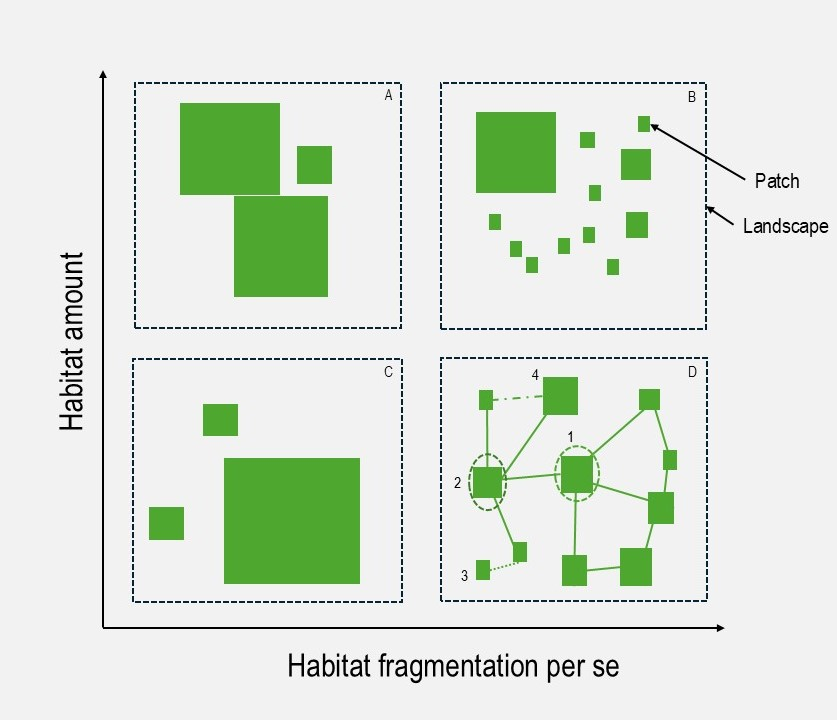
\includegraphics[width = .8\textwidth]{figures/intro/fragmentation.jpg}
\captionof{figure}{Illustration of the effects of habitat loss and fragmentation, adapted from \cite{fahrig_habitat_2019}, and of connectivity}
\label{fig:connectivity_intro}
\end{center}
\end{tcolorbox}
	
	
	 However, while property rights may be assigned, they can be notoriously hard to enforce in areas where regal functions are challenged: \textit{de facto} rights are assigned and enforced. In this case, the common nature of the resource may not be the main concern: local market concentration forces may outweigh overexploitation forces, even in the presence of some of form of open access \citep{damania_economics_2007}. 
Around the world, wildlife poaching and trade typically originates from organised crime groups, and is associated with different criminal activities \citep{mozer_introduction_2023}.  In those cases, concentrated markets tend to emerge and characterize wildlife markets, as competition is hindered by violent organised crime groups. \\
	At one extreme, locally monopolistic markets structure for wildlife products may emerge, especially in the case of endemic species (e.g. native and restricted to an area).
They may be the conservationists' bestfriend \citep{solow_resources_1974, hannesson_note_1983}, depending on specific, context dependent market and species characteristics, as a monopolist has an interest in restricting supply to increase prices, if consumers do not react too much (e.g. under limited demand elasticity). A vast range of  market structures \citep{damania_economics_2007, hannesson_effects_1985} sticking to real world situations have been studied. However, the full range of interactions between a species endemism, local market power, cost of effort and access to final consumer markets require more analysis to clarify the impact of market structure.\\
	Other drivers of overexploitation can be found in the large expected benefits (relative to other local economic activity) some natural resources can bear, most of the time because of their rarity (e.g. absence of economically viable substitute), whether today or in the future \citep{Kremer2000}. While the effects of substituting man-made products to disrupted ecosystem services are starting to get empirically studied \citep{frank_economic_2024} and show how dreadful costs can be, the effect of introducing substitutes to illegally poached wildlife products can be an example of strong substitutability between natural and man-made assets \citep{chen_economics_2017}. As broader forces affect overexploitation, including poverty, it is clear that adressing overexploitation implies generalizing conclusion from the interplay of a single species with the institutional setting, how a  species' future interacts with the availability of substitutes, and how the distribution of revenues from sustainable harvests may foster a reasoned use of the resource. 
	
	A wide range of policies have been implemented at different organisational levels, to jointly or separately halt the identifed drivers of biodiversity decline on land and at sea, with varying degrees of success. 




\subsection*{Policies for remedying the decline}
\addcontentsline{toc}{section}{Policies for remedying the decline}
\par

Successive international policy frameworks have sought to halt biodiversity loss by addressing its drivers comprehensively. In 2022, the 15th conference of the UN Convention on Biological Diversity launched the \href{https://www.cbd.int/doc/c/e6d3/cd1d/daf663719a03902a9b116c34/cop-15-l-25-en.pdf}{Keunming Montreal Global Biodiversity Framework (GBF)}, replacing the Strategic Plan for Biodiversity 2011-2020 and the Aichi Targets. The GBF sets four global goals for 2050, with 23 measurable targets to halt biodiversity loss by 2030. These goals include maintaining ecosystem integrity and connectivity and preventing human-induced extinctions (Goal A), sustainably using biodiversity (Goal B), sharing conservation benefits and burdens equitably (Goals C and D)\footnote{See \href{https://www.cbd.int/doc/c/e6d3/cd1d/daf663719a03902a9b116c34/cop-15-l-25-en.pdf}{Section G. Kunming-Montreal Global Goals for 2050}}. \href{https://www.cbd.int/gbf/targets/5}{Targets} include restoring 30\% of degraded ecosystems, conserving 30\% of land and sea areas, and ensuring the sustainable use and management of wild species.



%\begin{tcolorbox}[breakable, 
%colback=verylightgray, 
%colframe=gray!75!black,
%title={Box 3 - The Convention on Biological Diversity and the Aichi Targets},
%code={\singlespacing},
%fontupper=\small]
%\label{box:policy_frameworks_for_biodiv}
%\par % This \par ensures spacing before the text starts
%\justifying % Start justified text

%In 2010, the Convention on Biological Diversity set its "Strategic Plan for Biodiversity 2011-2020", structured around the 20 Aichi Biodiversity Targets, spanning over 5 goals :

%\begin{itemize}
%\item Goal A : Address the underlying causes of biodiversity loss by mainstreaming biodiversity across government and society
%\item Goal B : Reduce the direct pressures on biodiversity and promote sustainable use
%\item Goal C : To improve the status of biodiversity by safeguarding ecosystems, species and genetic diversity
%\item Goal D : Enhance the benefits to all from biodiversity and ecosystem services
%\item Goal E : Enhance implementation through participatory planning, knowledge management and capacity building
%\end{itemize}

%In 2020, the Global Biodiversity Outlook 5 \citep{global_biodiversity_outlook} showed that none of the Aichi %Target were globally met, and only 6 targets were partially achieved, including the identification and eradication of invasive species on islands, the setting of 17\% of terrestrial and inland water areas and 10\% of coastal and marine areas as conservation areas, the implementation of policy instruments and effective national biodiversity strategy and planning, and the increase in financing biodiversity protection. 

%While several elements showed progress, the failure of the 2011-2020 Strategic Plan was patent. Measurable indicators to assess progress towards targets were missing. This was tackled with the new Global Biodiversity Framework that took over in 2020, although with severe limitations. According to critics \citep{maron_setting_2021}, the current framework also lacks ecological scale-specific indicators (for genes, species, ecosystems) and do not provide specific net outcome statements (such as the 1.5C degree target of the Paris Agreements) across areas, nor a clear implementation timeline. 

%Additionally, the 2011-2020 Strategic Plan failed as countries did not have to report on their progress, only declare their targets. The 2020 Global Biodiversity Framework has implemented follow-up measures : although it is not a legally binding frameworks, countries who have signed commit to demonstrating progress towards the targets and update their National Biodiversity Strategy and Action Plans (see section B.5 and section J of the \href{https://www.cbd.int/doc/decisions/cop-15/cop-15-dec-04-en.pdf}{GBF})
%\end{tcolorbox}
Other international treaties, such as the \href{https://cites.org/fra}{Convention on International Trade in Endangered Species (CITES)} established in 1973, regulate trade in endangered species to prevent illegal wildlife trade\footnote{CITES features 183 member parties (countries), it lists species across "appendices", with varying degree of protection of the species and restrictions limiting the trade in endangered species.\\
Appendix 1 : the most endangered species, threatened with extinction and prohibited international trade, except when the purpose of exports is not commercial\\
Appendix 2 : species that are not necessarily now threatened with extinction but that may become so unless trade is closely controlled\\
Apppendix 3 : species included at the request of a Party that already regulates trade in the species and that needs the cooperation of other countries to prevent unsustainable or illegal exploitation} and promote species survival. Despite its scope, CITES’ effectiveness is debated. Local enforcement \citep{HEID2023102784} and demand reduction campaigns \citep{macfarlane_reducing_2022, moorhouse_demand_2024} are critical, but trade bans can sometimes increase prices and poaching incentives \citep{hsiang_does_2016}. In some cases, conservation farming has succeeded by “flooding the market” \citep{gentry_looking_2019, phelps_framework_2014, tensen_under_2016}. Supply-side interventions have occasionally succeeded at reducing poaching and recovering wild populations – e.g., vicuña and spotted cat \citep{iucn_world_2000, sahley_biological_2007} – but they have also failed – e.g., green python, African elephant \citep{lyons_wildlife_2011, hsiang_does_2016}. Uncertainty around conservation outcomes from market-based approaches has led to continued reliance on trade bans and controls that are often ineffective at reducing poaching.

National and supranational policies have also been key. In the U.S., policies like  \href{https://www.fs.usda.gov/Internet/FSE_DOCUMENTS/fseprd645666.pdf}{Wilderness Act of 1964} created protected areas to preserve habitats. In the wake of the environmentalist movement of the 1960s and 1970s, landmark regulations aimed at protecting natural habitats, such as the \href{https://www.epa.gov/laws-regulations/summary-clean-water-act}{Clean Water Act of 1972} (ensuring sewage to limit the disruption of wildlife habitat), and specifically targeted towards species conservation with the \href{https://www.fws.gov/sites/default/files/documents/endangered-species-act-accessible.pdf}{Endangered Species Act of 1973}. Results of the Endangered Species Act are debated. While the impacts seem to be overall positive on species recovery, budget dedicated to listings are slim , and the associated costs are substantial and concentrated on private landowners while benefits are more broadly distributed \citep{brown_economics_1998, langpap_economics_2018}
%
Localized initiatives, such as the \href{https://y2y.net/}{Yellowstone Yukon Conservation Initiative} (1993), connect ecological areas across the U.S. and Canada,using private conservation and local policy making. 
%
In Europe, the Natura 2000 network\footnote{A system of protected areas, established in application of the European Union Birds Directive (1976) and Habitats Directive (1992), and formally in place starting the mid 2000s} has created the largest conservation area globally, covering 18\% of land and 9\% of marine regions in the EU, across 28,000 sites. In broad strokes, it delineates conservation areas of ecological interest where development and human activities are restricted. Its ambition stemmed from taking into account the scale of biodiversity processes rather than administrative boundaries to develop an interconnected network of conservation areas. The ecological and economic performances of such a network are substantial, as they generate spatial spillovers both in terms of economic and ecological performance \citep{cocco_relaxing_2023}.

Acknowledging that biodiversity habitat can be seen as a continuum between unsuitable and suitable conditions, mechanisms such as Payments for Ecosystem Services (PES) are leveraged to incentivize conservation on agricultural land. Taking into account the ecological spillovers of decreased spillovers, payments for ecosystem services with agglomeration bonuses, such that neighbors gain an additional marginal benefit when a new local participant implements conservation measures, can be efficient \citep{parkhurst2002agglomeration, bareille_agglomeration_2023}. Overall, the spatial consequences of decentralized policies has yet to be fully integrated in policy making.

Finally, some policies aim at mitigating the threats posed by climate change on ecosystems and species, by changing landscape connectivity. In mediterranean forests, where biodiversity is exceptionally high but wildfires are an ever growing threat \citep{Dupuy2019ClimateCI, wasserman_climate_2023}, fuel treatment operations\footnote{Mechanical thinning, prescribed burns, and sometimes, logging, have been leveraged to decrease the fuel load in risky areas and theoretically decrease the probability and severity of burns upon wildfire occurence. In numerous regions, such as conifer forests in California \citep{Vaillant2009, Kalies2016, low_shaded_2023}, eucalypt forests in South Western Australia \citep{burrows2013, boer_long-term_2009, Florec2020}, southern Europe \citep{Fernandes2013}, evidence shows that fuel treatments, can mitigate wildfire intensity and spread. Land management agencies have historically implemented these policies in Australia \citep{burrows2013}, Europe, and the United States (and are projected to ramp up, for example under the Infrastructure Investment and Jobs Act of 2021 in the US)} limit the occurence and severity of wildfires. Public policy is leveraged in the face of increasing risk, limited insurability and threats to biodiversity. For example, with limited insurability of homes in the wildland urban interface in California\footnote{For example, \href{https://www.washingtonpost.com/climate-environment/2024/08/29/california-insurance-wildfires-allstate/}{200,000 homeowners will see an increase in their insurance premium} by an average of 34.1\% from Allstate insurance in November 2024. In 2023, the FAIR plan, designed to be the insurer of last resort in California (state mandated but privately funded) saw a \href{https://www.cfpnet.com/key-statistics-data/}{38.3\% increase in its total exposure.}}, as well as the potential economy-wide human and non-human damages from wildfires \citep{wang_economic_2021, heft-neal_behavior_2023, Ayars2023} state-mandated and operated fuel treatment policies are of the essence. However, with increased budgets and improved spatial planning, these policies could achieve better performances in reducing risk while protecting biodiversity.\\
Decentralized policy mechanisms exist, such as mandates to create a defensible buffer around individual properties : in California, a 100-foot defensible around houses is mandated in State Responsibility Areas,and can translate in reduced insurance premia;  in France, in dedicated regions, the "obligation de débroussaillement" mandates fuel control operations in a 50m radius to "decrease the intensity of wildfires and limit their spread"
\footnote{Translated by the author - \href{https://www.legifrance.gouv.fr/codes/article_lc/LEGIARTI000047809197}{Article L131-10} of the Code Forestier} with fines reaching $5,000$ euros for failing to comply.


I focus on the analysis of the interplay between biodiversity and human actions, through the NCPs it provides and the anthropogenic drivers of its decline. As existing policies have had varying degrees of success in halting biodiversity decline, a framework for policy design is required. I use \textit{economics} to jointly analyze the causes of this decline and provide policy recommendations. 


\subsection*{Biodiversity as an economic object}
\addcontentsline{toc}{section}{Biodiversity as an economic object}
The definition of economics has expanded with new methods and objects but primarily focuses on analyzing human behavior at individual and collective levels to manage scarce resources across alternatives \citep{mankiw_principles_2011, bade_foundations_2002, backhouse_retrospectives_2009}. This leads to two goals: understanding and explaining the state of the world (positive approach) and determining the best ways to manage resources (normative approach). Economics thus provides tools to analyze biodiversity loss and design policy.

However, applying economics to biodiversity is challenging. It requires commensurability of values, often through monetary valuation. Initially, biodiversity was valued for its products (hunting, fishing, logging) traded at market prices, focusing on resources in a specific state—dead. This approach captured only part of the "use value" of species \citep{Krutilla1967} (in the NCP framework, the material NCPs associated with food and materials), failing to consider their full value. Over time, the notion of "use value" expanded to include species' direct and indirect contributions. Many studies have used market proxies to estimate biodiversity's price\footnote{For instance, hedonic methods \citep{rosen_hedonic_1974} use variations in market prices for goods like real estate linked to environmental features, while the travel cost method \citep{clawson_economics_1967, bhandari_willingness_2010} measures consumer spending on experiences like wildlife viewing.}. Where market proxies fail, for lack of data for example, non-market valuation techniques have emerged \citep{carson_contingent_2012}, relying on stated preferences \footnote{For example, following the Exxon-Valdez spill in 1989, surveys were developed to estimate the value of affected biodiversity by asking people's willingness to pay for recovery \citep{carson_contingent_1992, arrow_report_1993, carson_contingent_2003}, though these methods are controversial \citep{Diamond94}}
%However, making the economics of biodiversity is not an easy task. 
%Management requires a commensurability of objects in terms of values (not necessarily with the same indicators, but a basis for rational comparison). Hence, a first step involves finding a common measurement, which has often implied monetary valuation. The valuation of biodiversity started with the valuation of its products :  hunting, fishing, logging have always been instrumental in human livelihoods, its products became economic objects to be traded with an established market price. This approach only considered said resources through a particular ontological state : dead. 
%Focusing on single species, this approach was only able to elicit the part of the "use value" of species (see \cite{Krutilla1967} and in the modern NCP framework, the material NCPs associated with food and materials) and not the integral value of species \citep{Krutilla1967}. The notion of "use value" had to be broadened to encompass the direct and indirect contributions of species, through a variety of techniques, and put a monetary value on them. A wealth of research has relied on market proxies, where market price for goods and services associated with biodiversity feature, were used to derive the price of biodiversity\footnote{On the one hand, hedonic methods \citep{rosen_hedonic_1974} have used the variation in observed market prices for a variety of goods, such as real estate, related to the variation of environmental and biodiversity features, and have studied how these variations have been internalized in goods market prices. On the other hand, methods such as the travel cost method \citep{clawson_economics_1967, bhandari_willingness_2010} have relied on observed consumer behavior and expenditures to experience "Nature", such as wildlife seeing, to elicit the price people are willing to pay for biodiversity}. When impossible to apply, for lack of proxy or data, other methods have relied on non-market valuation techniques \citep{carson_contingent_2012}, eliciting people's willingness to pay using stated preferences \footnote{For example, in 1989, the tanker Exxon-Valdez spilled close to 42 million liters of oil in Alaska, in an ecologically sensitive area : marine populations were decimated. According to \href{https://darrp.noaa.gov/oil-spills/exxon-valdez}{the National Oceanic and Atmospheric Administration}, an estimated 250,000 seabirds were killed, 2,800 sea otters, 22 killer whales, billions of salmons were killed. Numerous species are not in recovery after 25 years. In order to hold Exxon accountable, surveys were developped to assess the value of marine biodiversity, by surveying the willingness of people to pay for wildlife\citep{carson_contingent_1992, arrow_report_1993, carson_contingent_2003}, with controversed success \citep{Diamond94}}. 
With the ecosystem services framework, valuation techniques were scaled to capture various services \citep{Costanza1997}. Multiple methods extended biodiversity valuation across scales, from genetics to habitats and functions \citep{bartkowski_capturing_2015}.
Recently, approaches shifted from direct monetary metrics to assessing species' effects on outcomes like health \citep{frank_social_nodate,frank_economic_2024}. A significant body of research rejected monetary valuation, focusing instead on biodiversity metrics to weigh against economic outcomes \citep{Mouysset2011, Watzold2016a}. These metrics help assess or plan biodiversity evolution.

%With the rise of the ecosystem services framework, valuation techniques were developed at a broad scale to encompass the various services \citep{Costanza1997}. Overall, a variety of methods has been leveraged to extend the valuation of biodiversity at different scales, ranging from genetics to habitats, and encompassing functions \citep{bartkowski_capturing_2015}.
%In recent years, these approaches have been further developed by departing from direct monetary metrics, towards measuring the influence of species on other outcomes such as health \citep{frank_social_nodate,frank_economic_2024}. 
%A large strand of research refused to include direct monetary valuation, and chose to focus on biodiversity metrics to be weighed against monetary outcomes \citep{Mouysset2011, Watzold2016a}. These metrics can be used to assess the evolution of biodiversity, or to plan it. 

Managing biodiversity involves balancing alternatives while accounting for the specificity of living elements, regeneration and extinction rates, which requires understanding its temporal dynamics. Economics provides a framework to model these dynamics and assess the impact of different actions on current and future biodiversity. Models, as "stories with structure" \citep{GibbardVarian}, where the structure is "the logical and mathematical form of a set of postulates" with "elements of interpretation" \citep{GibbardVarian}, are used for a variety of purposes (see box 3).
Alongside the evolution of monetary valuation techniques, \textit{bioeconomic models} have been developed to design policies for resource management and biodiversity conservation.\\

%Weighing the different alternatives, across uses of biodiversity, across means of preserving it, requires factoring the specificity of biodiversity : regeneration rates are commensurable with human experience, and potentially, extinction rates. From an epistemological standpoint, this implies considering the temporal dimension of the resource. Economics provides an explicit framework to consider the temporal dynamic of biodiversity and the consequences of different actions on its current and future state through the use of models. Models are "stories with a specified structure", where the structure is "the logical and mathematical form of a set of postulates" with "elements of interpretation" \citep{GibbardVarian}. Using mathematics, models can be used for a variety of functions (see box 3). In an other strand of research, alongside the evolution of monetary valuation techniques, \textit{bioeconomic models} have been developed to design policies for resource management and biodiversity conservation.

\begin{tcolorbox}[breakable, 
colback=verylightgray, 
colframe=gray!75!black, 
title= {Box 3 - What do models do? },
%code={\singlespacing},
fontupper=\small]

 \cite{varenne_epistemologie_2014} furthers the "mediator" approach and labels models as facilitators, across multiple dimensions. A non-exhaustive typology of the roles models can play includes (i) a pedagogical role (facilitating communication), (ii) a predictive role (facilitating anticipation), (iii) a heuristic role (facilitating the explanation of a mechanism with a few simple interactions), (iv) prescriptive (facilitating the response to a given problem) and (iv) integrative (facilitating exchanges between disciplines). 

\end{tcolorbox}


\subsection*{Bioeconomic modeling for the study and management of biodiversity}
\addcontentsline{toc}{section}{Bioeconomic modeling for the study and management of biodiversity}
Bioeconomic models \citep{Gordon1954, smith_models_1969, clark_profit_1973} have emerged from joint efforts by economists and ecologists to manage resources accounting for the specific dynamics of biotic elements \citep{Parent_Mouysset_Missemer_Levrel_2024}. Bioeconomic models are analytical tools that jointly model the feedbacks between components of biodiversity in wild or weakly manageed ecosystems and economic activities, at different levels (e.g micro, mezzo and macro levels). 
Historically, the first bioeconomic models have emerged from population ecology and static economic analysis, to study the management of fisheries. The Gordon-Schaeffer model highlights the evolution of a fish population according to different harvest regimes, and aims at maximizing revenues in equilibrium. It distinguishes effort levels between those providing the maximum economic yield from those providing the maximum sustainable yield (e.g. resulting in the largest fish growth), yielding new policy perspectives: as the maximum sustainable yield effort is larger than the maximal economic yield, the policy target should be the former. Aiming for the maximum economic effort would therefore yield larger fish populations and promote economic efficiency. The original model was later extended to account for transitory dynamics and integrate elements from capital theory, focusing on the dynamic allocation of resources through time \citep{smith_models_1969, clark_profit_1973}. 

\begin{itemize}
\item Switch to land : other models focus on agricultural contexts and model the evolution of pests
\item Summary of first chapter:
\begin{itemize}
\item Bring MEY and MSY on land : the harvesting paradigm, swanson etc
\item Other approach : no longer monetize biodiversity and increase spatial granularity
\end{itemize}

\item Outline the evolution of bioeconomic modeling with economic models (e.g. taking into account risk and multiple players, as well as switching from pure optimality to more "positive" approaches) and ecological modeling
\item Gradual evolution of models to fulfill different functions of modeling or be different types of facilitators
\\
Box on ecological modeling : from population ecology to conservation and restoration ecology; change of scales, models integrate more and more spatial heterogeneity etc. 
\end{itemize}

\begin{tcolorbox}[breakable, 
colback=verylightgray, 
colframe=gray!75!black, 
title= {Box 3 - A brief overview of ecological modeling for biodiversity},
%code={\singlespacing},
fontupper=\small]
\par % This \par ensures spacing before the text starts
\justifying %
Ecology is a branch of biology that studies of the relationships between living organisms and their environment. 

While 


\end{tcolorbox}

\subsection*{Specific bioeconomic modeling challenges in the face of anthropogenic drivers}
\addcontentsline{toc}{section}{Specific bioeconomic modeling challenges in the face of anthropogenic drivers}

\begin{itemize}
\item Modelling challenges from the literature : 
\begin{itemize}
\item Integrate space in optimal management and focus on the role of space as an endogenous variable, not just spatial granularity
\item Take into account the full interplay of uncertainties : risk, uncertainty, how decision makers adapt etc. 
\item Operating a switch from population ecology to broader scale approaches that still integrate the dynamics of species, and not just static distributions with niches etc, such as landscape ecology and restoration ecology further
\item Integrate indigenous knowledge and perspecitves
\item Refine the study of intricate (to define more) market dynamics
\end{itemize}
\item Current challenges posed in relation with the challenges outlined in the conceptual part for remedy of overexploitation and habitat loss/fragmentation
\begin{itemize}
\item Integrating space in decision making : 
\begin{itemize}
\item deal with non convexity of objective function; 
\item Optimization on discrete landscapes : cannot use continuity
\item Dimensionality curse : dynamic programming fails, at least when performed brutely, so need to trade (i) temporal depth of planning, (ii) extent of space and (iii) complexitiy of ecological mechanisms. 
\item 
\end{itemize}
\item Refine the study of dynamics with heterogeneous and strategic players:
\begin{itemize}
\item Integrate more the roles of ecological and economic heterogeneity through land : limited scope for analytical tractability, need to resort to numerical methods
\item Interaction on a same market of different types of actors, with strategic responses : complicated choice variables in terms of game theory, as exploitation and decision over space are related; 
\end{itemize}
\item Need a variety of perspectives for models to be helpful for decision making : integrating both a positive approach (e.g. compare policy scenarios in a second best world) and a normative approach to guide policy. 
\end{itemize}
\end{itemize}

\subsection*{Research questions}
\addcontentsline{toc}{section}{Research questions}

\begin{itemize}
\item Remind the NCPs I'm focusing on :
\begin{itemize}
\item NCP1 - Habitat creation and maintenance : "the formation and continued production, by ecosystems, of ecological conditions necessary or favorable for living beings important to humans"
\item NCP10 - Regulation of organisms detrimental to humans : "regulation, by ecosystems or organisms, of pests, pathogens, predators, competitors, parasites and potentially harmful organisms"
\item NCP13 - Materials and assistance : "production of materials derived from organisms in cultivated or wild ecosystems and direct use of living organisms for decoration, transport, company and labour"
\end{itemize}
 
How can we adress these drivers jointly, as they share common and specific drivers
\item How can we improve bioeconomic mdodeling to improve policy design that focuses on space and market dynamics? 
\begin{itemize}
\item Can we modernize existing tools to adress pressing policy challenges, in the case of CITES
\item Can we bring new tools (graph theory for example) and perspectives to improve management of space overall, especially in the case of conflicting NCPs? 
\item How can we endogenize decisions over the management of space? 
\end{itemize}
\item Remind the scales of biodiversity : how can we integrate the various scales of biodiversity together, and take full advantage of advances in ecology? 
\end{itemize}

\section*{Dissertation outline}
\addcontentsline{toc}{section}{Dissertation outline}
\subsubsection*{Thematic divide of the dissertation}

\begin{table}[H]
\centering

\begin{tabular}{c|c|c}
Driver & Habitat loss, fragmentation& Overexploitation \\
       &  and connectivity   & / underharvest \\
\hline
Chapter 2      & \cellcolor{verylightgray}                    &                                \\
\hline
Chapter 3      & \cellcolor{verylightgray}                    & \cellcolor{verylightgray}      \\
\hline
Chapter 4      &                                              & \cellcolor{verylightgray}   \\   
\hline
\end{tabular}
\end{table}


\subsubsection*{Adressing different scale of biodiversity}


\begin{table}[H]
\centering

\begin{tabular}{c|c|c|c}
Driver &  Biodiversity level & Ecology perspective  & Unit of analysis \\
\hline
Chapter 2      &  Community         &             Landscape ecology                   & Spatial \\
\hline
Chapter 3      &  Population        &  Population ecology   \\
               &                    & and landscape ecology & individuals (biomass stock \\
			   & 				   &  metapopulations  &  and spatial flow) \\
\hline
Chapter 4      &      Population    & Population ecology  & individuals (stock)   \\   
\hline
\end{tabular}
\end{table}

\subsubsection*{Using different model functions and focusing on different methodological challenges}

Explain the data v. theory divide
\begin{table}[H]
\centering

\begin{tabular}{c|c|c}
Driver &  Decision prism  & Model use   \\
\hline
Chapter 2      &  Social planner         &   Prescrptive and pedagogical   \\
\hline
Chapter 3      &  Social planner and decentralized &  Illustrative, pedagogical  \\
\hline
Chapter 4      &      Second best    & Prescriptive and? \\   
\hline
\end{tabular}
\end{table}


\begin{table}[H]
\centering

\begin{tabular}{|c|c|c|}
Driver & \textbf{Space} & \textbf{dynamics}\\
\hline
Chapter 2      &            &                 \\
\hline
Chapter 3      &           &        \\
			  &                     &   \\
\hline
Chapter 4      &          &   \\   
\hline
\end{tabular}
\end{table}

%% Global biodiversity decline : why should we care?

%% Conceptual challenges



